\documentclass[../main.tex]{subfiles}

\begin{document}
\chapter{Combinatorial Search}
So far, we have learned the most fundamental search strategies on general data structures such as array, linked list, graph, and tree. In this chapter, instead of searching on explicit and well defined data structures, we extend and discuss more \textit{exhaustive search} algorithms that can solve rather obscure and challenging \textit{combinatorial problems}, such as sudoku and the famous Travels Salesman Problem. For combinatorial problems, we have to figure out the potential search space, and rummage a solution. 
\section{Introduction}
Combinatorial search problems consists of $n$ items and a requirement to find a solution, i.e., a set of $L < N$ items that satisfy specified conditions or constraints. For example, a sudoku problem where a $9\times 9$ grid is partially filled with number between 1 and 9, fill the empty spots with numbers that satisfy the following conditions:
\begin{figure}[!ht]
    \centering
    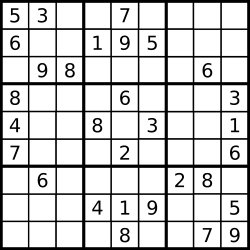
\includegraphics[width= 0.35\columnwidth]{fig/250px-Sudoku-by-L2G-20050714.png}
    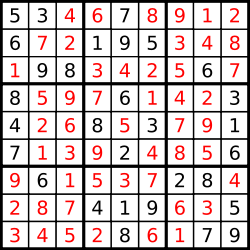
\includegraphics[width= 0.35\columnwidth]{fig/250px-Sudoku-by-L2G-20050714_solution.png}
    \caption{A Sudoku puzzle and its solution}
    \label{fig:backtrack_puzzle_1}
\end{figure}
\begin{enumerate}
    \item Each row has all numbers form 1 to 9.
    \item Each column has all numbers form 1 to 9.
    \item Each sub-grid ($3 \times3$) has all numbers form 1 to 9.
\end{enumerate}
This sudoku together with one possible solution is shown in Fig.~\ref{fig:backtrack_puzzle_1}. In this case, we have $81$ items, and we are required to fill 51 empty items with the above three constraints. 
\paragraph{Model Combinatorial Search Problems} 
We can model the combinatorial search solution as a vector $s = (s_0, s_1, ..., s_{L-1})$, where each variable $s_i$ is selected from a finite  set $A$, which is called the \textit{domain} for each variable. Such a vector might represent an arrangement where $s_i$ contains the i-th item of a permutation, in the combination problem, a boolean denotes if the i-th item is selected already, or it can represent a path in a graph or a sequence of moves in a game. In the sudoku problem, each $s_i$ can choose from a number in range $[1, 9]$.


\paragraph{Problem Categories} Combinatorial search problems arise in many areas of computer science such as artificial intelligence, operations search, bioinformatics, and electronic commerce. These problems typically involve finding a \textit{grouping}, \textit{ordering}, or \textit{assignment} of a discrete, finite set of objects that satisfy given conditions or constraints.  We introduce two well-studied types of problems that are more likely to be NP-hard and of at least exponential complexity:
% in computer science mainly studies algorithms that solve exponential or even NP-hard problems, such as:
\begin{enumerate}
    \item Constraint Satisfaction Problems (CSP) are mathematical questions defined as a set of variables whose state must satisfy a number of constraints or limitations(mathematical equations or inequations), such as Sudoku, N-queen, map coloring, Crosswords, and so on. The size of the search space of CSPs can be roughly given as:
    \begin{align}
        O(cd^L)
    \end{align}
    Where there are $L$ variables, each with domain size $d$, and there are $c$ constraints to check out. 
    \item Combinatorial optimization problems consist of searching for maxima or minima of an objective function $F$ whose domain is a discrete but large configuration space.  Some classic examples are:
    \begin{itemize}
        \item Travelling Salesman Problems (TSP): given position $(x, y)$ of $n$ different cities, find the shortest possible path that visits each city exactly once.
        \item Integer Linear Programming: maximize a specified linear combination of a set of integers $X_1, .., X_{n}$ subject to a set of linear constraints each of the form:
        \begin{align}
            a_1X_1 + ... + a_{n}X_{n} \leq c
        \end{align}
        \item Knapsack Problems: Given a set of items, each with a weight and a value, determine the number of each item to include in a collection so that the total weight is less than or equal to a given limit and the total value is as large as possible.
    \end{itemize}
\end{enumerate}


\paragraph{Search Strategies} From Chapter Discreet Programming, we have learned the basic enumerative combinatorics, including counting principles and knowledge on permutations, combinations, partitions, subsets, and subsequences. Combinatorial Search builds atop this subject, and together through different search strategies such as depth-first search and best-first search, it is able to enumerate the search space and find the solution(s)  with necessary speedup methods. In this chapter, we only discuss about complete search and only acknowledge the existence of approximate search techniques. 

\textit{Backtracking} is a process of depth-first based search where it ``builds'' the search tree on the fly incrementally instead of having a tree/graph structure beforehand  to search through. Backtracking fits to solve combinatorial search problems because:
\begin{enumerate}
    \item It is space efficient for the usage of a DFS and the candidates are built incrementally and their validity to fit a solution is checked right away.
    \item It is time efficient for that some partial candidates can be pruned if the algorithm believes that it will not lead to our final complete solution. 
\end{enumerate}

 Because the ordering of variables $s_0, ..., s_{L-1}$ can potentially affect the size of the search space sometimes. Thus, backtracking search relies on one or more heuristics to select which variable to consider next. \textit{Look-ahead} is one such heuristic that is preferably applied to check the effects of choosing a given variable to evaluate or to decide the order of values to give to it. 
 
 There are other Breath-first Search based strategies that might work better than backtracking, such as  for combinatorial optimization problems, best-first branch and bound search might be more efficient than its depth-first counterpart. 

\paragraph{Speedups}

The speedup methods are well studied in computer science, and we list two general ways to prune unqualified or unnecessary branches during the search of backtracking:
\begin{enumerate}
    \item Branch and Prune: This method prunes the unqualified branches with constraints of the problems. This is usually applied to solve constraint restricted problems (CSPs).
    \item Branch and Bound: This method prunes unnecessary branches via comparing an estimation of a partial candidate with a found global best solution. If the estimation states that the partial candidate will never lead us to a better solution, we cut off this branch. This technique can be applied to solve a general optimization problems, such as Travel Salesman Problems (TSP), knapsack problems, and so.
\end{enumerate}
% To notice that these speedup techniques are general for searching, not specifically for Backtracking. For example, branch and bound often be linked to best-first search. 

\section{Backtracking}
In this section, we first introduce the technique of backtracking, and then demonstrate it by implementing common enumerative combinatorics seen in Chapter Discreet Programming. 
\subsection{Introduction}
Backtracking search is an exhaustive search algorithm(depth-first search) that systematically assigns all possible combinations of values to the variables and checks if these assignments constitute a solution. Backtracking is all about choices and consequences and it shows the following two properties:
 \begin{enumerate}
     \item \textbf{No Repetition and Completion:} It is a systematic generating method that enumerates all possible states exactly at most once: it will not miss any valid solution but  avoids repetitions. If there exists  ``correct'' solution(s), it is guaranteed to be found. This property makes it ideal for solving combinatorial problems where the search space has to be constructed  and enumerated. Therefore, the worst-case running time of backtracking search is exponential with the length of the state ($b^L$, $b$ is the average choice for each variable in the state).% such as combination and permutation which requires us to enumerate all possible solutions. We focus on demonstrating this property in this section. 
    \item \textbf{Search Pruning:} Along the way of working with partial solutions, in some cases, it is possible for us to decide if they will  lead to a valid \textit{complete solution}. As soon as the algorithm is confident to say the partial configuration is either invalid or nonoptimal,  it abandons this  \textit{partial candidate}, an then ``backtracks'' (return to the upper level), and resets to the upper level's state so that the search process can continue to explore the next branch for the sake of efficiency.  This is called \textit{search pruning} with which  the algorithm ends up amortizely visiting each vertex less than once.  This property makes backtracking the most promising way to solve CSPs and combinatorial optimization problems. 
 \end{enumerate}

Solving sudoku problem with backtracking algorithm, each time at a level in the DFS,  it tries to extend the last partial solution $s = (s_0, s_1, ..., s_{k})$ by trying out all 9 numbers at $s_{k+1}$, say we choose 1 at this step. It  testifies the partial solution with the desired solution:
\begin{enumerate}
    \item If the partial solution $s = (s_0, s_1, ..., s_{k}, 1)$ is still valid, move on to the next level and work on trying out $s_{k+2}$.
    \item If the partial solution is invalid and is impossible to lead to a complete solution, it ``backtracks'' to the last level and resets the state as $s = (s_0, s_1, ..., s_{k})$ so that it can try our other choices if there are some left(which in our example, we will try $s_{k+1}=2$) or keep ``backtracking'' to even upper level.
\end{enumerate}
The process should be way clearer once we have learned the examples in the following subsections. 

\subsection{Permutations}
Given a list of items, generate all possible permutations of these items. If the set has duplicated items, only enumerate all unique permutations.
\subsubsection{No Duplicates(L46. Permutations)} When there are no duplicates, from Chapter Discreet Programming, we know the number of all permutations are:
\begin{equation}
    p(n, m) = \frac{n!}{(n-m)!}
\end{equation}
where $m$ is the number of items we choose from the total $n$ items to make the permutations. 
\begin{lstlisting}[numbers=none]
For example:
a = [1, 2, 3]
There are 6 total permutations:
[1, 2, 3], [1, 3, 2],
[2, 1, 3], [2, 3, 1],
[3, 1, 2], [3, 2, 1]
\end{lstlisting}
\paragraph{Analysis} Let us apply the philosophy of backtracking technique. We have to build a state with length $3$, and each variable in the state has three choices: 1, 2, and 3. The constraint here comes from permutation which requires that no two variables in the state will be having the same value. To build this incrementally with backtracking, we state with an empty state \texttt{[]}. At first, we have three options, we get three partial results $[1], [2]$, and $[3]$. Next, we handle the second variable in the state: for $[1]$, we can choose either 2 or 3,getting $[1,2]$ and $[1,3]$; same for $[2]$, where we end up with $[2,1]$ and $[2,3]$; for $[3]$, we have $[3,1]$ and $[3,2]$. At last, each partial result has only one option, we  get all permutations as shown in the example. We visualize this incrementally building candidates in Fig.~\ref{fig:backtrack_permutation}. 
\begin{figure}[h]
    \centering
    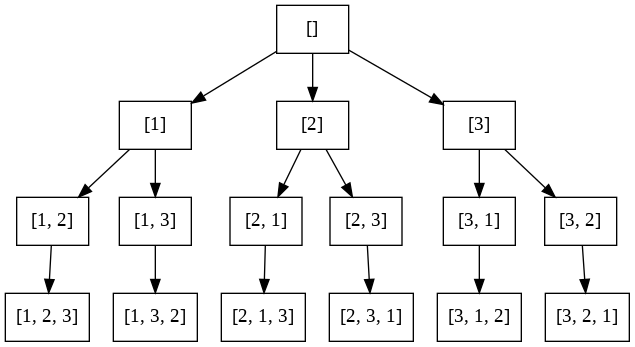
\includegraphics[width= 0.8\columnwidth]{fig/permutation.png}
    \caption{The search tree of permutation}
    \label{fig:backtrack_permutation}
\end{figure}

However, we only managed to enumerate the search space, but not systematically or recursively with the Depth-first search process. With DFS, we depict the traverse order of the vertexes in the virtual search space with red arrows in Fig.~\ref{fig:backtrack_permutation}. The backward arrows mark the ``backtracking'' process, where we have to reset the state to the upper level. 

\paragraph{Implementation} We  use a list of boolean \texttt{bUsed} to track which item is used in the search process. 
\texttt{n} is the total number of items, \texttt{d} is the depth of the depth-first search process, \texttt{curr} is the current state, and \texttt{ans} is to save all permutations. The following code, we generate $p(n, m)$
\begin{lstlisting}[language=Python]
def p_n_m(a, n, m, d, used, curr, ans):
  if d == m: #end condition
    ans.append(curr[::]) 
    return
  
  for i in range(n):
    if not used[i]:
      # generate the next solution from curr
      curr.append(a[i])
      used[i] = True
      print(curr)
      # move to the next solution
      p_n_m(a, n, m, d + 1, used, curr, ans)
      #backtrack to previous partial state
      curr.pop()
      used[i] = False
  return
\end{lstlisting}
Check out the running process in the source code.

\paragraph{Alternative: Swapping Method}   
\begin{figure}[h]
    \centering
    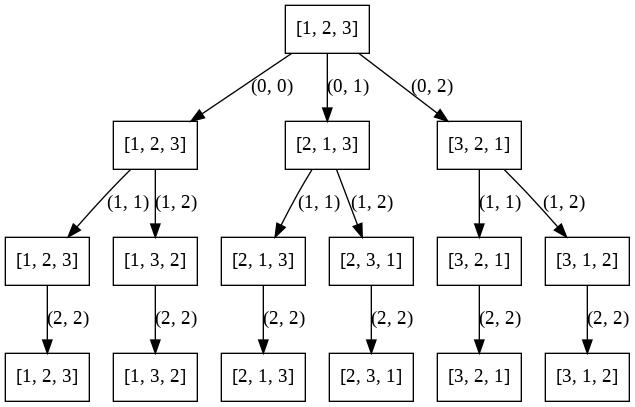
\includegraphics[width= 0.8\columnwidth]{fig/permutation_swap.png}
    \caption{The search tree of permutation by swapping. The indexes of items to be swapped are represented as a two element tuple. }
    \label{fig:backtrack_permutation_swap}
\end{figure}
We first start with a complete state, such that $s=[1, 2, 3]$ in our case. By swapping $1$ and $2$, we get $[2, 1, 3]$ and $[2, 3, 1]$ can be obtained by swapping $1$ and $3$ on top of $[2, 1, 3]$. With all permutations as leaves in the search space, the generating process is similar to Fig.~\ref{fig:backtrack_permutation}. We show this alternative process in Fig.~\ref{fig:backtrack_permutation_swap}. At first, we swap index 0 with all other indexes, including 0, 1, and 2. At the second layer, we move on to swap index 1 with all other successive indexes, and so on for all other layers.  The Python code is as:
\begin{lstlisting}[language=Python]
ans = []
def permutate(a, d):
  global ans
  if d == len(a):
    ans.append(a[::])
  for i in range(d, len(a)):
    a[i], a[d] = a[d], a[i]
    permutate(a, d+1)
    a[i], a[d] = a[d], a[i]
  return
\end{lstlisting}
There is Johnson-Trotter algorithm that utilizes such swapping method, which avoids recursion, and instead computes the permutations by an iterative method. 
\subsubsection{With Duplicates(47. Permutations II)}
We have already know that $p(n, n)$ is further decided by the duplicates within the $n$ items. Assume we have in total of $d$ items are repeated, and each item is repeated $x_i$ times, then the number of all arrangements $pd(n, n)$ are:
\begin{align}
    pd(n, n) &= \frac{p(n, n)}{x_0!x_1!...x_{d-1}}, \\
    \texttt{w.r.t } & \sum_{i=0}^{d-1} x_i \leq n
\end{align}
For example, when $a = [1, 2, 2, 3]$, there are $\frac{4!}{2!}$ unique permutations, which is 12 in total, and are listed as bellow:
\begin{lstlisting}[numbers=none]
[1, 2, 2, 3], [1, 2, 3, 2], [1, 3, 2, 2],
[2, 1, 2, 3], [2, 1, 3, 2], [2, 2, 1, 3],
[2, 2, 3, 1], [2, 3, 1, 2], [2, 3, 2, 1],
[3, 1, 2, 2], [3, 2, 1, 2], [3, 2, 2, 1]
\end{lstlisting}
\paragraph{Analysis} 
\begin{figure}[h]
    \centering
    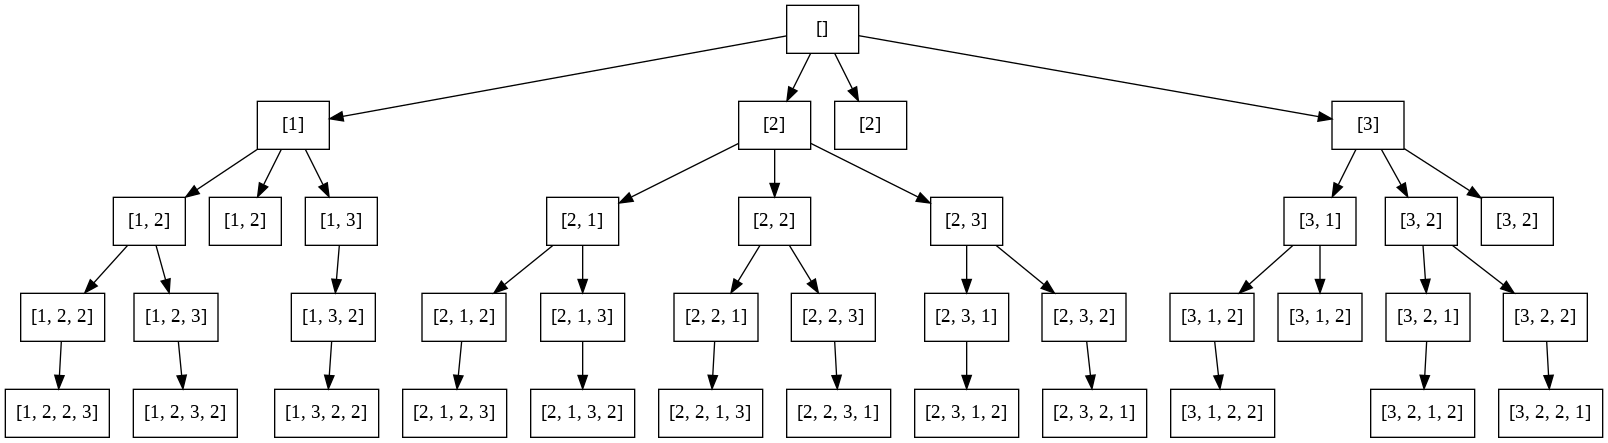
\includegraphics[width= 1.2\columnwidth]{fig/permutation_repeat.png}
    \caption{The search tree of permutation with repetition}
    \label{fig:backtrack_permutation_duplicates}
\end{figure}
The enumeration of these all possible permutations can be obtained with backtracking exactly the same as if there are no duplicates. However, this is not efficient since it has doubled the search space with repeated permutations. Here comes to our first time applying the Branch and Prune method:  we avoid repetition by pruning off redundant branches. 

One main advantage of backtracking is not to save all intermediate states, thus we should find a mechanism that avoids generating these intermediate states at the first place.  One solution is that we sort all $n$ items, making all repeat items adjacent to each other. We know if the current intermediate state is redundant by simply comparing this item with its predecessor: if it equals, we move on from building state with this item to the next item in line. The search tree of our example is shown in Fig.~\ref{fig:backtrack_permutation_duplicates}. 

\paragraph{Implementation} The implementation is highly similar to previous standard permutation code other than three different points: 
\begin{enumerate}
\item Before the items are called by \texttt{permutate}, they are sorted first.
\item  A simple condition check to avoid generating repeat states.
    \item We used a dictionary data structure \texttt{tracker} which has all unique items as keys and each item's corresponding occurrence as values to replace the boolean vector \texttt{used} for slightly better space efficiency.
\end{enumerate}
The Python code is as:
\begin{lstlisting}[language=Python]
from collections import Counter
def permuteDup(nums, k):
    ans = []
    def permutate(d, n, k, curr, tracker):  
      nonlocal ans 
      if d == k:
          ans.append(curr)
          return
      for i in range(n):
          if tracker[nums[i]] == 0:
            continue
          if i - 1 >= 0 and nums[i] == nums[i-1]:
              continue
          tracker[nums[i]] -= 1
          curr.append(nums[i])

          permutate(d+1, n, k, curr[:], tracker)
          curr.pop()
          tracker[nums[i]] += 1
      return
    
    nums.sort()
    permutate(0, len(nums), k, [], Counter(nums))
    return ans
\end{lstlisting}

\begin{bclogo}[couleur = blue!30, arrondi=0.1,logo=\bccrayon,ombre=true]{Can you extend the swap method based permutation to handle duplicates?} 
\end{bclogo}

\subsubsection{Discussion}
From the example of permutation, we have demonstrated how backtracking works to construct candidates with an implicit search tree structure: the root node is the initial state, any internal node represents intermediate states, and all leaves are our candidates which in this case there are $n!$ for $p(n, n)$ permutation. In this subsection, we want to point out the unique properties and its computational and space complexities.
\paragraph{Two Passes} Backtracking builds an implicit search tree on the fly, and it does not memorize any intermediate state. It visits the  vertices
 in the search tree in two passes: 
 \begin{enumerate}
     \item Forward pass: it builds the solution incrementally and reaches to the leaf nodes in a DFS fashion. One example of forward pass is $[]->[1]->[1,2]->[1,2,3]$.
     \item Backward pass: as the returning process from recursion of DFS, it also backtracks to previous state. One example of backward pass is $[1,2,3]->[1,2],->[1]$. 
 \end{enumerate}First, the forward pass to build the solution \textbf{incrementally}.
The change of \texttt{curr} in the source code indicates all vertices and the process of backtracking, it starts with $[]$ and end with $[]$. This is the core character of backtracking. We print out the process for the example as:
\begin{lstlisting}[numbers=none]
[]->[1]->[1, 2]->[1, 2, 3]->backtrack: [1, 2]
backtrack: [1]
[1, 3]->[1, 3, 2]->backtrack: [1, 3]
backtrack: [1]
backtrack: []
[2]->[2, 1]->[2, 1, 3]->backtrack: [2, 1]
backtrack: [2]
[2, 3]->[2, 3, 1]->backtrack: [2, 3]
backtrack: [2]
backtrack: []
[3]->[3, 1]->[3, 1, 2]->backtrack: [3, 1]
backtrack: [3]
[3, 2]->[3, 2, 1]->backtrack: [3, 2]
backtrack: [3]
backtrack: []
\end{lstlisting}

\paragraph{Time Complexity of Permutation}
In the search tree of permutation in Fig.~\ref{fig:backtrack_permutation}, there are in total $V$ nodes, which equals to $\sum_{i=0}^{n}{p_{n}^{k}}$. Because in a tree the number of edges $|E|$ is $|v|-1$, making the time complexity $O(|V|+|E|)$ the same as of $O(|V|)$. Since $p(n, n)$ itself alone takes $n!$ time, making the permutation an NP-hard problem. 

\paragraph{Space Complexity} A standard depth-first search consumes $O(bd)$ space in worst-case to execute, where $b$ is branching factor and $d$ is the depth of the search tree. In the combinatorial search problems, usually depth and branching is decided by the total number of variables in the state, making $b \sim d \sim n$. In backtracking, we have space complexity $O(n^2)$. However, in normal standard DFS, the input--tree or graph data structure--is given and not attributed to space complexity. For a NP-hard combinatorial search problem, this input is often exponential. Backtracking search outcompetes the standard DFS by avoiding such space consumption; it only keeps a dynamic data structure(\texttt{curr})  to construct node on the fly.  % The slight different can be critical for problems with large state description.  

\subsection{Combinations}
Given a list of $n$ items, generate all possible combinations of these items. If the input has duplicated items, only enumerate unique combinations. 
\subsubsection{No Duplicates (L78. Subsets
)}
From Chapter Discrete Programming, we list the powerset--all $m$-subset, $m\in[0, n]$ as:
\begin{align}
    C(n, m) = \frac{P(n, m)}{P(m, m)} = \frac{n!}{(n-m)!m!}
\end{align}
For example, when $a=[1, 2, 3]$, there are in total $7$ $m$-subsets, they are:
\begin{lstlisting}[numbers=none]
C(3, 0): []
C(3, 1): [1], [2], [3]
C(3, 2): [1, 2], [1, 3], [2, 3]
C(3, 3): [1, 2, 3]
\end{lstlisting}
\paragraph{Analysis} 
\begin{figure}[!ht]
    \centering
    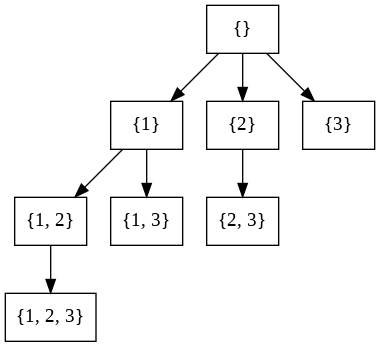
\includegraphics[width= 0.5\columnwidth]{fig/combination.png}
    \caption{The Search Tree of Combination.}
    \label{fig:backtrack_combination}
\end{figure}
We can simply reuse the method of permutation, but with a problem that it generates lots of duplicates. For example, $P(3, 2)$ includes $[1, 2]$ and $[2, 1]$ which are indeed the same subset. Of course, we can check redundancy with saved $m$-subsets, but its not ideal. A systematical solution that avoids duplicates all along is preferred. If we limit the items we put into the $m$-subsets to be only increasing(of indexes of items or of values of items), in which case $[2, 1]$, $[3,1]$, and $[3,2]$ will never be generated. The enumeration of combination through backtracking search is shown in Fig.~\ref{fig:backtrack_combination}.

\paragraph{Implementation} Two modifications based on permutation code:
\begin{enumerate}
    \item \texttt{for} loop: in the loop to iterate all possible candidates, we limit the candidates to be having larger indexes only.
    \item We do not have to use a data structure to track the state of each candidate because any candidate that has larger index is a valid candidate.
\end{enumerate}
We use \texttt{start} to track the starting position of valid candidates. The code of combination is:
\begin{lstlisting}[language=Python]
def C_n_k(a, n, k, start, d, curr, ans):
  if d == k: #end condition
    ans.append(curr[::]) 
    return
  
  for i in range(start, n):    
    curr.append(a[i])
    C_n_k(a, n, k, i+1, d+1, curr, ans)
    curr.pop()
  return
\end{lstlisting}

\paragraph{Alternative: 0 and 1 Selection} We have discussed that a powerset written as $P(S)$. With each item either being appear or not appear in the resulting set makes the value set $\{0, 1\}$, resulting $|P(S)| = 2^n$. Follow this pattern, with our given example, we can alternatively generate a powerset like this:
\begin{lstlisting}[numbers=none]
s   sets
1   {1}, {}
2   {1,2}, {1}, {2}, {}
3   {1,2,3}, {1,2}, {1, 3}, {3}, {2, 3}, {2}, {3}, {}
\end{lstlisting}
This process can be better visualized in a tree as in Fig.~\ref{}. We can see this process results $2^n$ leaves compared with our previous implementation which has a total of $2^n$ nodes is slightly less efficient. The code is as:
\begin{lstlisting}[language=Python]
def powerset(a, n, d, curr, ans):
  if d == n:
    ans.append(curr[::]) 
    return

  # Case 1: select item
  curr.append(a[d])
  powerset(a, n, d + 1, curr, ans)
  # Case 2: not select item
  curr.pop()
  powerset(a, n, d + 1, curr, ans)
  return
\end{lstlisting}

\paragraph{Time Complexity} The total nodes within the implicit search space of combination shown in Fig.~\ref{fig:backtrack_combination} is $\sum_{k=0}^{n}C_{n}^{k} =2^n$, which was explained in Chapter Discreet Programming. Thus, the time complexity of enumerating the powset is $O(2^n)$ and is less compared with $O(n!)$ that comes with the permutation.

\paragraph{Space Complexity} Similarly, combination with backtracking search uses slightly less space. But, we can still acclaim the upper bound to be $O(n^2)$. 

\subsubsection{With Duplicates(L90. Subsets II)}
 Assume we have $m$ unqiue items, and the frequency of each is marked as $x_i$, with $\sum_{i=0}^{m-1}x_i = n$. 
\begin{align}
\sum_{k=0}^{n} c(n, k) = \prod_{i=0}^{m-1}(x_i + 1)
\end{align}

For example, when $a=[1, 2, 2, 3]$, there are $2\times 3 \times 2 = 12$ combinations in the powerset, they are listed as bellow:
\begin{lstlisting}[numbers=none]
[], [1], [2], [3], [1, 2], [1, 3], [2, 2], [2, 3],
[1, 2, 2], [1, 2, 3], [2, 2, 3],
[1, 2, 2, 3]
\end{lstlisting}
However, counting $c(n, k)$ with duplicates in the input replies on the specific input with specific distribution of these items. We are still able to count by enumerating with backtracking search. 
\paragraph{Analysis and Implementation} The enumeration of the powerset with backtracking search is the same as handling the iterations of choice in the enumeration of permutation with duplicates. We first sort our items in increasing order of the values. Then we replace the \texttt{for} loop from the above code with the following code snippet to handle the repetition of items from the input:
\begin{lstlisting}[language=Python]
  for i in range(start, n): 
    if i - 1 >= start and a[i] == a[i-1]:
              continue   
    ...
\end{lstlisting}
\subsection{More Combinatorics}
In this section, we supplement more use cases of backtracking search in the matter of other types of combinatorics. 
\subsubsection{All Paths in Graph}
\begin{figure}[ht!]
    \centering
    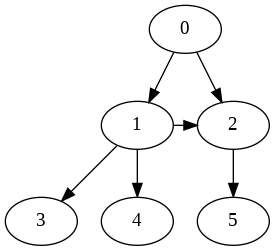
\includegraphics[width=0.4\columnwidth]{fig/all_path_demo.png}
    \caption{Acyclic graph}
    \label{fig:my_label}
\end{figure} 
For a given acyclic graph, enumerate all paths from a starting vertex $s$. For example, for the graph shown in Fig.~\ref{fig:my_label}, and a starting vertex $0$, print out the following paths:
\begin{lstlisting}[numbers=none]
0, 0->1, 0->1->2, 0->1->2->5, 0->1->3, 0->1->4, 0->2, 0->2->5
\end{lstlisting}
\paragraph{Analysis} The backtracking search here is the same as how to apply a DFS on an explicit graph, with rather one extra point: a state $path$ which might have up to $n$ items ( the total vertices of a graph). In the implementation, the \texttt{path} vector will dynamically be modified to track all paths constructed as the go of the DFS. The code is offered as:
% Backtracking technique can be naturally used in graph path traversal. One example is to find all possible paths from a source to the target. One simpler occasion is when the graph has no cycles. Backtrack technique can enumerate all paths in the graph exactly once for each. 

% The implementation is as follow: we still use dfs, because there has no cycles, we have no need to track the visiting state of each node. We generate the possible answer with backtracking technique through the \texttt{path} variable to track each state. 
\begin{lstlisting}[language=Python]
def all_paths(g, s, path, ans):
  ans.append(path[::])
  for v in g[s]:
    path.append(v)
    all_paths(g, v, path, ans)
    path.pop()
\end{lstlisting}
You can run the above code in the Goolge Colab to see how it works on our given example.
% Feed in the above network and run the following code:
% \begin{lstlisting}[language=Python]
% al = [[1], [2], [4], [], [3, 5], [6], []]
% ans = []
% path = [0]
% all_paths(al, 0, path, ans)
% \end{lstlisting}
% With the printing, we can see the whole process, \texttt{path} changes as the description of backtrack. \begin{lstlisting}[numbers=none]
% [0, 1]
% [0, 1, 2]
% [0, 1, 2, 4]
% [0, 1, 2, 4, 3]
% [0, 1, 2, 4] backtrack
% [0, 1, 2, 4, 5]
% [0, 1, 2, 4, 5, 6]
% [0, 1, 2, 4, 5] backtrack
% [0, 1, 2, 4] backtrack
% [0, 1, 2] backtrack
% [0, 1] backtrack
% [0] backtrack
% \end{lstlisting}
% We can see each state, we can always have a matching backtrack state. 
% \begin{bclogo}[couleur = blue!30, arrondi=0.1,logo=\bccrayon,ombre=true]{What to do if there is a cycle?} 
% \end{bclogo}

\subsubsection{Subsequences(940. Distinct Subsequences II)} Given a string, list all unique subsequences. There may or may not exist duplicated characters in the string. For example, when $s='123'$, there are in total 7 subsequences, which are:
\begin{lstlisting}[numbers=none]
'', '1', '2', '3', '12', '13', '23', '123'
\end{lstlisting}
When $s='1223'$ which comes with duplicates, there are 12 subsequences:
\begin{lstlisting}[numbers=none]
'', '1', '2', '3', '12', '13', '22', '23', 
'122', '123', '223',
'1223'
\end{lstlisting}
\paragraph{Analysis} From Chapter Discrete Programming, we have explained that we can count the number of unique subsequences through recurrence relation and pointed out the relation of subsquences with subsets(combinations). Let the number of unique subsequences of a sequence as $seq(n)$ and the number of unique subsets of a set as $set(n)$ with $n$ items in the input. All subsequences are within subsets, and the subsequence set has larger cardinality than subsets, $|seq(n)|\geq |set(n)|$. From the above example, we can also see that when there are only unique items in the sequence or when there are duplicates but all duplicates of an item are adjacent to each other:
\begin{itemize}
    \item The cardinality of subsequences and subsets equals, $|seq(n)= set(n)|$.
    \item The subsequences and subsets share the same items when the ordering of the subsequences are ignored. 
\end{itemize}
This indicates that the process of enumerating subsequences is almost the same as of enumerating a powerset. This should give us a good start.

\paragraph{Implementation} However, if we change the ordering of the duplicated characters in the above string as $s='1232'$, there are in total 14 subsequences instead:
\begin{lstlisting}[numbers=none]
'', '1', '2', '3', '12', '13', '23', '22', '32',
'123', '122', '132', '232',
'1232'
\end{lstlisting}
\begin{figure}[!ht]
    \centering
    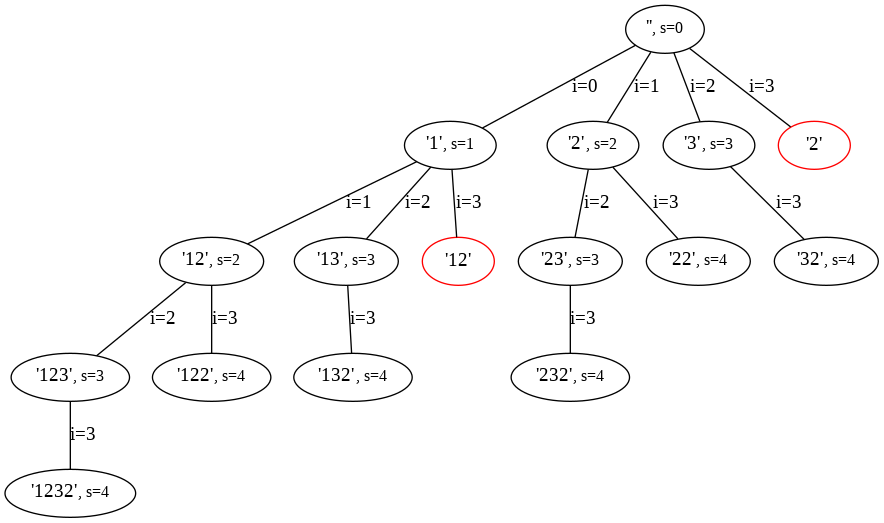
\includegraphics[width= 1.0\columnwidth]{fig/subsequence.png}
    \caption{The Search Tree of subsequences.The red circled nodes are redundant nodes. Each node has a variable $s$ to indicate the starting index of candidates to add to current subsequence. $i$ indicate the candidate to add to the current node.}
    \label{fig:backtrack_subsequence}
\end{figure}
Therefore, our code to handle duplicates should differ from that of a powerset.  In the case of powerset, the algorithm first sorts items so that all duplicates are adjacent to each other, making the checking of repetition as simple as checking the equality of item with its predecessor. However, in a given sequence, the duplicated items are not adjacent most of the time, we have to do things differently. We draw the search tree of enumerating all subsequences of string ``1232'' in Fig.~\ref{fig:backtrack_subsequence}. From the figure, we can observe that to avoid redundant branches, we simply check if a current new item in the subsequence is repeating by comparing it with all of its predecessors in range $[s, i]$. The code for checking repetition is as:
\begin{lstlisting}[language=Python]
def check_repetition(start, i, a):
  for j in range(start, i):
    if a[i] == a[j]:
      return True
  return False
\end{lstlisting}
And the code to enumerate subsequences is:
\begin{lstlisting}[language=Python]
def subseqs(a, n, start, d, curr, ans):
  ans.append(''.join(curr[::])) 
  if d == n: 
    return
  
  for i in range(start, n):  
    if check_repetition(start, i, a):
      continue    
    curr.append(a[i])
    subseqs(a, n, i+1, d+1, curr, ans)
    curr.pop()
  return
\end{lstlisting}

 

\subsection{Backtracking in Action}
So far, we have applied backtracking search to enumerate combinatorics. In this section, we shall see how  backtracking search along with search pruning speedup methods solve two types of challenging NP-hard problems: Constraint Satisfication Problems (CSPs) and Combinatorial Optimization Problems. 

As we have briefly introduced the speedup methods needed to solve larger scale of CSPs and COPs. For example, assume within the virtual search tree, the algorithm is currently at level 2 with state $s=[s_0, s_1]$. If there are $c$ choices for state $s_1$, and if one choice is testified to be invalid, this will prune off $\frac{1}{c}$ of the whole search space. In this section, we demonstrate backtracking search armored with Branch and Prune method solving CSPs and Branch and Bound solving COPs.


\section{Solving CSPs}
Officially, a constraint satisfaction problem(CSP) consists of a set of $n$ variables, each denoted as $s_i$, $i\in[0, n-1]$; their respective value domains,  each denoted as $d_i$; and a set of $m$ constraints, each denoted as $c_j$, $j \in [0, m-1]$. A \textit{solution} to a CSP is an assignment of values to all the variables such that no constraint is violated. A \textit{binary} CSP is one in which each of the constraints involves at most two variables. A CSP can be represented by a \textit{constraint graph} which has a node for each variable and each constraint, and an arc connecting variable nodes contained in a constraint to the corresponding constraint node.

We explain a few strategies from the CSP-solver's arsenal that can potentially speedup the process:
\begin{enumerate}
    \item Forward Checking: The essential idea is that when a variable $X$ from $s_i$ is instantiated with a value $x$ from its domain $d_i$, the domain of each future uninstantiated variable $Y$ is examined. If a value $y$ is found such that $X=x$ conflicts with $Y=y$, then $y$ is temporarily removed from the domain of $Y$. 
    \item Variable Ordering: The order in which variables are considered while solving a CSP method can have a substantial impact on the search space. One effective ordering is always select the next variable with the smallest remaining domain. In a dynamic variable ordering, the order of variables is determined as the search progresses, and often goes with forward checking which keeps updating the uninstantiated variables' domains. Selecting variable with the minimal domain first can pinpoint the solution quickly given the fact that the branch is still early on, and branch pruning at this stage is more rewarding. Another reasoning is that each step, when we are multiplying $d_i$ to the cost, we are adding the least expensive one, making this a greedy approach. 
\end{enumerate}
\subsubsection{Sudoku (L37)} 
\begin{figure}[!ht]
    \centering
    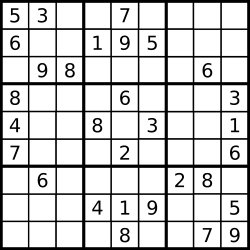
\includegraphics[width= 0.35\columnwidth]{fig/250px-Sudoku-by-L2G-20050714.png}
    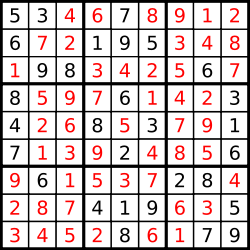
\includegraphics[width= 0.35\columnwidth]{fig/250px-Sudoku-by-L2G-20050714_solution.png}
    \caption{A Sudoku puzzle and its solution}
    \label{fig:backtrack_puzzle_2}
\end{figure}
A Sudoku grid shown in Fig.~\ref{fig:backtrack_puzzle_2} is a $n^2\times n^2$ grid, arranged into $n$ $n\times n$ mini-grids each containing the values $1,...,n$ such that no value is repeated in any row, column (or mini-grid).  
\paragraph{Search Space}
First, we analyze the number of distinct states in the search space which relies on how we construct the intermediate states and  our knowledge in Enumerative combinatorics. We discuss two different formulations on $9 \times 9$ grid:
\begin{enumerate}
    \item For each empty cell in the puzzle, we create a set by taking values $1, ..., 9$ and removing from it those values that appear as a given in the same row, column, or mini-grid as that cell. Assume we have $m$ spots and the corresponding candidate set of each spot is $c_i$, and initial cost estimation can be obtained which is:
    \begin{align}
        T(n) = \prod_{i=0}^{m-1} c_i
    \end{align}
    \item Each row can be presented by a 9-tuples, there will be 9 rows in total, resulting 9 9-tuples to represent the search state. With $c_i$ as the number of non-given values in the i-th 9-tuples, there are $c_i!$ ways of ordering these values by permuting.The number of different states in the search space is thus:
    \begin{align}
        T(n) = \prod_{i=0}^{8} c_i!
    \end{align}
\end{enumerate}
The two different ways each takes a different approach to formulate the state space, making its corresponding backtracking search differs too. We mainly focus on the first formulation with backtracking search.
\paragraph{Speedups} 
% \begin{figure}[h]
%     \centering
%     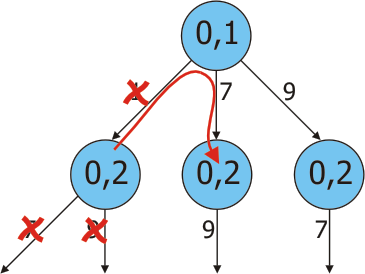
\includegraphics[width= 0.5\columnwidth]{fig/sudoku_backtracking.png}
%     \caption{Partial search tree of Sudoku in Fig.~\ref{fig:backtrack_puzzle_2}}
%     \label{fig:backtrack_sudoku}
% \end{figure}
Assume we have known all empty spots(variables) to fill in and we construct the search tree using backtracking. In our source code, we did an experiment comparing the effect of ordering variables with minimal domain first rule with arbitrary ordering. The experiment shows that the first method is more than 100 times faster than the second solving the our exemplary Sudoku puzzle. Therefore, we decide to always select the variable that has the least domain set to proceed next in the backtracking.

Further, we apply forward checking, for the current variable and a value we are able to assign, we recompute all the remaining empty spots' domain sets, and use the updated domain sets to decide:
\begin{itemize}
    \item If this assigment will lead to empty domain for any of other remaining spots, and if so, we terminate the search and backtrack.
    \item The spot to select next time with the ordering rule we choose. 
\end{itemize}
\paragraph{Implementation} We set aside three vectors of length 9,  \texttt{row\_state}, \texttt{col\_state}, and \texttt{block\_state} to track the state of all 9 rows, columns, and grids. The list has \texttt{set()} data structures as items, saving the numbers filled already in that row, col, and grid respectively. Two stages in the implementation:
\begin{enumerate}
    \item Initialization: We scan the whole each spot in the $9\times 9$ grid to record the states of the filled spots and to find all empty spots that waiting to be filled in.  With $(i,j)$ to denote the position of a spot, it corresponds to \texttt{row\_state[i]}, \texttt{col\_state[j]}, and \texttt{block\_state[i//3][j//3]}. We also write two functions to set and reset state with one assignment in the backtracking. The Python code is as follows:
\begin{lstlisting}[language=Python]
from copy import deepcopy
class Sudoku():
  def __init__(self, board):
    self.org_board = deepcopy(board)
    self.board = deepcopy(board)
    
  def init(self):
    self.A = set([i for i in range(1,10)])
    self.row_state = [set() for i in range(9)]
    self.col_state = [set() for i in range(9)]
    self.block_state = [[set() for i in range(3)] for i in range(3)]
    self.unfilled = []

    for i in range(9):
      for j in range(9):
          c = self.org_board[i][j]
          if c == 0:
              self.unfilled.append((i, j))
          else:
              self.row_state[i].add(c)
              self.col_state[j].add(c)
              self.block_state[i//3][j//3].add(c)
  
  def set_state(self, i, j, c):
    self.board[i][j] = c
    self.row_state[i].add(c)
    self.col_state[j].add(c)
    self.block_state[i//3][j//3].add(c)
    
  def reset_state(self, i, j, c):
    self.board[i][j] = 0
    self.row_state[i].remove(c)
    self.col_state[j].remove(c)
    self.block_state[i//3][j//3].remove(c)
\end{lstlisting}

\item Backtracking search with speedups:  In the initialization, we have another variable $A$ used as the domain set of the current processing spot. To get the domain set according to the constraints, a simple set operation is executed as: $A-(row\_state[i]|col\_state[j]|block\_state[i//3][j//3])$. In the solver, each time, to pick a spot, we first update all remaining spots in the \texttt{unfilled} and then choose the one with minimal domain. This process takes $O(n)$ which is trivial compared with the cost of the searching, with $9$ for computing domain set of a single spot, $9n$ for $n$ spots, and adding another $n$ to $9n$ to choose the one with the smallest size. The solver is implemented as:
\begin{lstlisting}[language=Python]
  def _ret_len(self, args):
    i, j = args
    option = self.A - (self.row_state[i] | self.col_state[j] | self.block_state[i//3 ][j//3])
    return len(option)
    
  def solve(self):
    if len(self.unfilled) == 0:
      return True
    # Dynamic variables ordering
    i, j = min(self.unfilled, key = self._ret_len)
    # Forward looking
    option = self.A - (self.row_state[i] | self.col_state[j] | self.block_state[i//3 ][j//3])
    if len(option) == 0:
      return False
    self.unfilled.remove((i, j))
    for c in option:
      self.set_state(i, j, c)
      if self.solve():
        return True
      # Backtracking
      else:
        self.reset_state(i, j, c)
    # Backtracking
    self.unfilled.append((i, j))
    return False
\end{lstlisting}
\end{enumerate}


\section{Solving Combinatorial Optimization Problems}
% Combinatorial optimization problems are characterized by an \textit{input}, i.e., a general description of conditions and parameters, and an \textit{objective} defining 

Combinatorial optimization is an emerging field at the forefront of combinatorics and theoretical computer science that aims to use combinatorial techniques to solve discrete optimization problems.  From a combinatorics perspective, it interprets complicated questions in terms of a fixed set of objects about which much is already known: sets, graphs, polytopes, and matroids. From the perspective of computer science, combinatorial optimization seeks to improve algorithms by using  mathematical methods either to reduce the size of the set of possible solutions or to make the search itself faster. 

Genuinely, the inner complexity of a COP is at least of exponential, and its solutions fall into two classes: exact methods and heuristic methods. In some cases, we may be able to find efficient exact algorithms with either greedy algorithms or dynamic programming technique such as finding the shortest paths on a graph can be solved by the Dijkstra (greedy) or Bellman-Ford algorithms(dynamic programming) to provide exact optimal solutions in polynomial running time. For more complex problems, COP can be mathematically formulated as a Mixed Linear Programming(MILP) model and which is generally solved using a linear-programming based branch-and-bound algorithm.  But, in other cases no exact algorithms are feasible, and the following randomized heuristic search algorithms though we do not cover in this section should be applied:
\begin{enumerate}
    \item Random-restart hill-climbing.
    \item Simulated annealing.
    \item Genetic Algorithms.
    \item Tabu search.
\end{enumerate}

\paragraph{Model Combinatorial Optimization Problems} It is a  good practice to formulate COPs with mathematical equations/inequations, which includes  three steps:
\begin{enumerate}
    \item Choose the decision variables that typically encode the result we are interested in, such that in a superset problem, each item is a variable, and each variable includes two decisions: take or not take, making its value set as ${0, 1}$.
    \item Express the problem constraints in terms of these decision variables to specify what the feasible solutions of the problem are.
    \item Express the objective function to specify the quality of each solution.
\end{enumerate}
There are generally many ways to model a COP.


\paragraph{Branch and Bound} Branch and bound (BB, B$\&$B, or BnB) is an algorithm design paradigm for discrete and combinatorial optimization problems, as well as mathematical optimization. A branch-and-bound algorithm consists of a systematic enumeration of candidate solutions by means of state space search: the set of candidate solutions is thought of as forming a rooted tree with the full set at the root. The algorithm explores branches of this tree, which represent subsets of the solution set. Before enumerating the candidate solutions of a branch, the branch is checked against upper and lower estimated bounds on the optimal solution, and is discarded if it cannot produce a better solution than the best one found so far by the algorithm. ``Branching'' is to split problem into a number of subproblems, and ``bounding'' is to find an optimistic estimation of the best solution to the the subproblems to either maximize the upper bound or minimize the lower bound.  To get the optimistic estimation, we have to \textit{relax constraints}.  In this section, we will exemplify both the minimization(TSP) and maximization problem(Knapsack). 

\paragraph{Search Strategies} In practice, we can apply different search strategies to enumerate the search space of the problem, such as depth-first, best-first, and least-discrepancy search. The way of how each listed strategy is applied in the combinatorial optimization problems is:
\begin{itemize}
    \item Depth-First: it prunes when a node estimation is worse than the best found solution.
    \item Best-First: it selects the node with the best estimation among the frontier set to expand each time. Worst scenario, the whole search tree have to be saved as long the best estimation is extremely optimistic and not a single branch is pruned in the process. 
    \item Least-Discrepancy: it trusts a greedy heuristic, and then move away from the heuristic in a very systematic fashion. 
\end{itemize}

In this section, we discuss exact algorithms using Branch and Bound with a variation of search strategies. During the interviews, questions that have polynomial exact solutions are more likely to appear, proving your mastery of dynamic programming or greedy algorithms design methodologies. However, it is still good to discuss this option. 

%%%%%%%%%%%%%%%%%%%%
\subsection{Knapsack Problem}
% In this section we want to showcase more searching strategies applied in solving optimization problems: comparing backtracking and a chance to use best-first search strategy. 

Given $n$ items with weight and value indicated by two vectors $W$ and $V$ respectively. Now, given a knapsack with capacity $c$, maximize the value of items selected into the knapsack with the total weight being bounded by $c$. Each item can be only used at most once. For example, given the following data, the optimal solution is to  choose item 1 and 3, with total weight of 8, and optimal value of 80.
\begin{lstlisting}[numbers=none]
c = 10
W = [5, 8, 3]
V = [45, 48, 35]
\end{lstlisting}
\paragraph{Search Space} In this problem, $x_i$ denotes each item, and $w_i$, $v_i$ for its corresponding weight and value, with $i\in[0, n-1]$. Each item can either be selected or left behind, indicating $x_i\in{0, 1}$. The selected items can not exceed the capacity, making $\sum_{i=0}^{n-1} w_i x_i \leq c$. And we capture the total value of the selected items as $\sum_{i=0}^{n-1} v_i x_i$.  Putting it all together:
\begin{align}
    \max_{v, x} \quad & \sum_{i=0}^{n-1} v_i x_i\\
    \textrm{s.t.} \quad  & \sum_{i=0}^{n-1} w_i x_i \leq c\\
    & x_i\in{0, 1}
\end{align}
With each variable having two choices, our search space is as large as $2^n$.

\paragraph{Branch and Bound} 

To bound the search, we have to develop a heuristic function to estimate an optimistic--maximum--total value a branch can lead to. 

In the case of knapsack problem, the simplest estimation is summing up the total values of selected items so far, and estimate the maximum value by adding the accumulated values of all remaining unselected items along the search. 

% And a branch is checked 
% \begin{align}
%     \texttt{if } estimate < found, 
% \end{align}

A tighter heuristic function can be obtained with \textbf{constraint relaxation}. By relaxing the condition of simply choose $\{0, 1\}$ to $[0, 1]$, that a fraction of an item can be chosen at any time. By sorting the items by the value per unit $\frac{v_i}{w_i}$, then a better estimate can be obtained by filling the remaining capacity of knapsack with unselected items, with larger unit value first be considered. A branch is checked on the optimal solution so far against the lower estimated bound in our case, and is discarded if it cannot produce a better solution than the best one found so far by the algorithm. Both heuristic functions are more optimistic compared with the true value, but the later is a tighter bound, being able to prune more branches along the search and making it more time efficient. We demonstrate branch and bound with two different search strategies: DFS(backtracking) and Best-First search.



% the items while the capacity is not exhausted, then select a fraction of the last item to fill the remaining capacity, which is a closer estimate of the real one but still optimisitc compared with selecting the remaining items.  What if we are allowed to get part of an item, so that we can fit the knapsack as full as possible. We can sort the items by their unit value, and take items in the order of decreasing unit values. Another bool vector is used to indicate if a certain item can be used or not. At first, all items are allowed, we can get an estimation of 92 in this case. For branches that decide not to take an item, that item is excluded using the bool vector.  We compare the estimation with the best found value, if the estimated value will never be better, then this branch will prunned. 


\subsubsection{Depth-First Branch and Bound}
\begin{figure}[h]
    \centering
    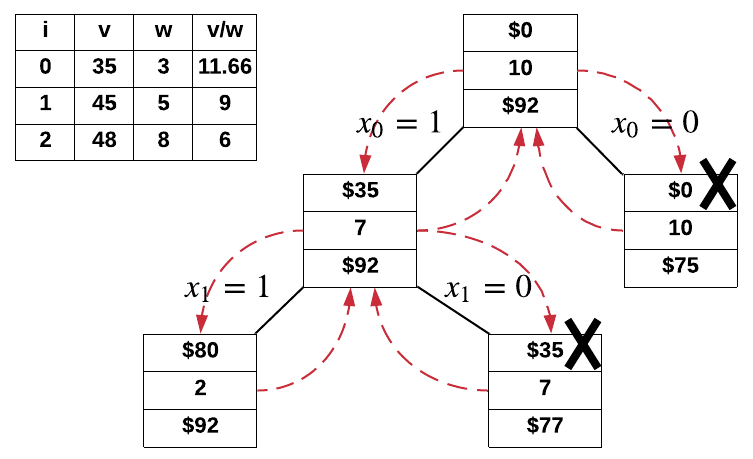
\includegraphics[width= 0.98\columnwidth]{fig/branch_and_bound_backtracking.png}
    \caption{Depth-First Branch and bound}
    \label{fig:knapsack_backtracking}
\end{figure}
We set up a class \texttt{BranchandBound} to implement this algorithm. First, in the initiation, we add additional $\frac{v_i}{w_i}$ to mark each item's value per unit, and sort these items by this value in decreasing order. Second, we have a function \texttt{estimate} which takes three parameters: \texttt{idx} as start index of the remaining items, \texttt{curval} is the total value based on all previous decision, and \texttt{left\_cap} as the left capacity of the knapsack. The code snippet is:
\begin{lstlisting}[language=Python]
import heapq

class BranchandBound:
  def __init__(self, c, v, w):
    self.best = 0 
    self.c = c
    self.n = len(v)
    self.items = [(vi/wi, wi, vi) for _, (vi, wi) in enumerate(zip(v, w))]
    self.items.sort(key=lambda x: x[0], reverse=True)

  def estimate(self, idx, curval, left_cap):
    est = curval
    # use the v/w to estimate
    for i in range(idx, self.n):
      ratio, wi, _ = self.items[i]
      if left_cap - wi >= 0: # use all
        est += ratio * wi
        left_cap -= wi
      else: # use part
        est += ratio * (left_cap)
        left_cap = 0 
    return est
\end{lstlisting}
In the Depth-first search process, it consists of two main branches: one considering to choose the current item, and the other to handle the case while the item is not selected. For the first branch, it has to be bounded by the capacity and the comparison of the best found solution against to the estimation. Additional \texttt{status} is to assist to visualize the process of the search, which tracks the combination of items. The process is shown in Fig.~\ref{fig:knapsack_backtracking}.  And the code is as:
\begin{lstlisting}[language=Python]
  def dfs(self, idx, est, val, left_cap, status):
      if idx == self.n:
        self.best = max(self.best, val)
        return
      print(status, val, left_cap, est )
      
      _, wi, vi = self.items[idx]
      # Case 1: choose the item
      if left_cap - wi >= 0: # prune by constraint
        # Bound by estimate, increase value and volume
        if est > self.best:   
          status.append(True)
          nest = self.estimate(idx+1, val+vi, left_cap - wi)   
          self.dfs(idx+1, nest, val+vi, left_cap - wi, status)
          status.pop()

      # Case 2: not choose the item
      if est > self.best:
        status.append(False)
        nest =  self.estimate(idx+1, val, left_cap)
        self.dfs(idx+1, nest, val, left_cap, status) 
        status.pop()
      return
\end{lstlisting}
\subsubsection{Best-First Branch and Bound}
Within Best-First search, we use priority queue with the estimated value, and each time the one with the largest estimated value within the frontier set is expanded first. Similarly, with branch and bound, we prune branch that has estimated value that would never surpass the best solution up till then. The search space is the same as in   Fig.~\ref{fig:knapsack_backtracking} except that the search process is different from depth-first. In the implementation, the priority queue is implemented with a min-heap where the minimum value is firstly popped out, thus we use the negative estimated value to make it always pop out the largest value conveniently instead of write code to implement a max-heap. 
\begin{lstlisting}[language=Python]
  def bfs(self):
      # track val, cap, and idx is which item to add next
      q = [(-self.estimate(0, 0, self.c), 0, self.c, 0)] # estimate, val, left_cap, idx
      self.best = 0
      while q:
        est, val, left_cap, idx = heapq.heappop(q)
        est = -est
        _, wi, vi = self.items[idx]
        if idx == self.n - 1:
          self.best = max(self.best, val)
          continue
        
        # Case 1: choose the item
        nest = self.estimate(idx + 1, val + vi, left_cap - wi)
        if nest > self.best:
          heapq.heappush(q, (-nest, val + vi, left_cap - wi, idx + 1))

        # Case 2: not choose the item
        nest = self.estimate(idx + 1, val, left_cap)
        if nest > self.best:
          heapq.heappush(q, (-nest, val, left_cap, idx + 1))
      return 
\end{lstlisting}

\subsection{Travelling Salesman Problem}
\begin{figure}[!ht]
    \centering
    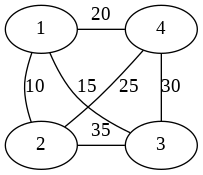
\includegraphics[width= 0.4\columnwidth]{fig/tsp_graph.png}
    \caption{A complete undirected weighted graph.}
    \label{fig:tsp_graph}
\end{figure}
Given a set of cities and the distances between every pair, find the shortest possible path that visits every city exactly once and returns to the origin city. For example, with the graph shown in Fig.~\ref{fig:tsp_graph}, such shortest path is $[0, 1, 3, 2, 0]$ with a path weight $80$. 
% \begin{lstlisting}[numbers=none]
% Assume our graph is a two dimensional list:
% g = [[(1, 10), (2, 15), (3, 20)], 
%   [(0, 10), (2, 35),(3,25)],
%   [(0, 15),(1,35),(3,30)],
%   [(0,20),(1,25),(2,30)]]
% g[0][0]=(1,10), means the edge between 0 and 1 with cost 10.
% \end{lstlisting}

\paragraph{Search Space} In TSP, a possible complete solution is a \textit{Hamiltonian cycle}, a graph cycle that visits each vertex exactly once. Since it is a cycle, it does not matter where it starts. For convenience, we choose vertex $0$ as the origin city. Therefore, in our example, our path starts and ends at $0$, and the remaining $n-1$ vertices between will  be a permutation of these vertices, making the complexity as $(n-1)!$. 

Because this is a complete graph, it might be tempting to apply backtracking on the graph to enumerate all possible paths and find and check possible solutions. However, this path searching will build a $n-1$-ary search tree with height equals to $n-1$, making the complexity as $\frac{(n-1)^{n}-1}{n-2}$, which is larger than the space of permutation among $n-1$ items. Therefore, in our implementation, we apply backtracking to enumerate all permutations of $n-1$ vertices and check its corresponding cost.  

\paragraph{Speedups} Since we only care about the minimum cost, then any partial result that has cost larger than the  minimum cost of all known complete solutions can be prunned. This is the \textit{Branch and bound} method that we have introduced that is often used in the combinatorial optimization. 
% solution is path with vertices forming a cycleneed to construct a list of vertices (\texttt{path}) and its total cost (\texttt{cost}) of all edges between as the state $s=(p, c)$, $p, c$ is short for path and cost respectively. A possible complete solution for path will have $n+1$ vertices which start with a vertex and end with the same, and $n-1$ vertices in between. Now, put together about constraints.
% \begin{itemize}
%     \item ``Visits every city exactly once'' means the first vertex will be a permutation of all cities, we get $n!$ combination (the last vertex does not matter).
%     \item We have $n!$ possible states. We can further spot redundant states. For a cycle, it does not matter where it starts, it is always the same cycle. For convenience, we choose vertex $0$ as the starting path, and there will only be $n-1$ vertex to permutate with, making the size of the state space to $(n-1)!$. 
%     \item We only care about the minimum cost, then any partial result that has cost larger than the  minimum cost of all known complete solution can be prunned. This is called \textit{Branch and bound} method, which is the extension of backtracking into the optimization problems.
% \end{itemize}

\paragraph{Implementation}  We built the graph as a list of dictionaries, each dictionary stores the indexed vertex's other cites and its corresponding distance as key and value respectively. Compared with standard permutation with backtracking, we add four additional variables: \texttt{start} to track the starting vertex, \texttt{g} to pass the graph to refer the distance information, \texttt{mincost} to save the minimum complete solution so far found, and \texttt{cost} to track the current partial path's cost. The code is shown as: 
\begin{lstlisting}[language=Python]
def tsp(a, d, used, curr, ans, start, g, mincost, cost):
  if d == len(a): 
    # Add the cost from last vertex to the start
    c = g[curr[-1]][start]
    cost += c
    if cost < mincost[0]:
      mincost[0] = cost
      ans[0] = curr[::] + [start]
    return
  
  for i in a:
    if not used[i] and cost + g[curr[-1]][i] < mincost[0] :
      cost += g[curr[-1]][i]
      curr.append(i)
      used[i] = True      
      tsp(a, d + 1, used, curr, ans, start, g, mincost, cost)
      curr.pop()
      cost -= g[curr[-1]][i]
      used[i] = False
  return
\end{lstlisting}
TSP is a NP-hard problem, and there is no known polynomial time solution so far.



\subsubsection{Other Solutions}
Whenever we are faced with optimization, we are able to consider the other two algorithm design paradigm--Dynamic Programming and Greedy Algorithms. In fact, the above two problems both have its corresponding dynamic programming solutions: for knapsack problem, polynomial solution is possible; for TSP, though it is still of exponential time complexity, it is much better than $O(n!)$. We will further discuss these two problems in Chapter Dynamic Programming. 
\section{Exercises}
\begin{enumerate}
\item 77. Combinations
\item 17. Letter Combinations of a Phone Number
\item 797. All Paths From Source to Target
    \item N-bit String: enumerate all n-bit strings with backtracking algorithm, for example:
\begin{lstlisting}[numbers=none]
n = 3, all 3-bit strings are:
000, 001, 010, 011, 100, 101, 110, 111
\end{lstlisting}
\item 940. Distinct Subsequences II
\item N-queen
\item Map-coloring
\item 943. Find the Shortest Superstring (hard). Can be moduled as traveling salesman problem and dynamic programming
\end{enumerate}
\end{document}